\section{Testy}

Gotowe implementacje algorytmów, po testach weryfikujących poprawność ich działania, zostały również sprawdzone na kilku rzeczywistych zbiorach danych pobranych z repozytorium UCI \cite{UCI}.
Dla każdego zbioru wykonano wyszukiwanie zamkniętych zbiorów częstych dla wsparć z zakresu od 0.1 do 0.9 ze skokiem 0.1.
W większości testów wygrywał algorytm Charm, ale nie zawsze.

Zbiór Mushroom ma wymiary 8125 wierszy na 23 atrybuty. 
W tym przypadku oba algorytmy zachowywały się podobnie, ale bezsprzecznie wydajniejszy okazał się Charm - rysunek \ref{plot:mushroom}.

Dużo mniejszym zbiorem jest zbiór House o wymiarach 91 wierszy na 17 kolumn.
Według tego testu \ref{plot:house} nadal Charm jest lepszy. 
Szczególnie dla najmniejszego testowanego wsparcia Clotest działał zdecydowanie za długo.

Ale dla zbioru z dwukrotnie większą liczbą atrybutów w porównaniu do powyższych zachowanie powoli się zmienia \ref{plot:promotor}. Kolejnym testowanym jest zbiór Promotor o wymiarach 106 wierszy na 58 kolumn.
Nadal nie jest to duży zbiór (pod względem liczby wierszy).
Ale przewaga algorytmu Charm została przełamana.

Idąc dalej w tym kierunku przetestowany został zbiór Splice-jxn o wymiarach 3190 wierszy na 61 kolumn.
Tym razem to algorytm Closet zdecydowanie lepiej się sprawdza \ref{plot:slice}.
Algorytm Charm dla wsparć poniżej 0.5 był na tyle wolny, że dla czytelności nie uwzględniono tych punktów na wykresie.

Podsumowując, według naszych testów implementacja algorytmu Closet zachowuje się lepiej względem Charm w przypadku zbioru danych o większej liczbie atrybutów.

\begin{figure}
\caption{Test dla zbioru Mushroom}
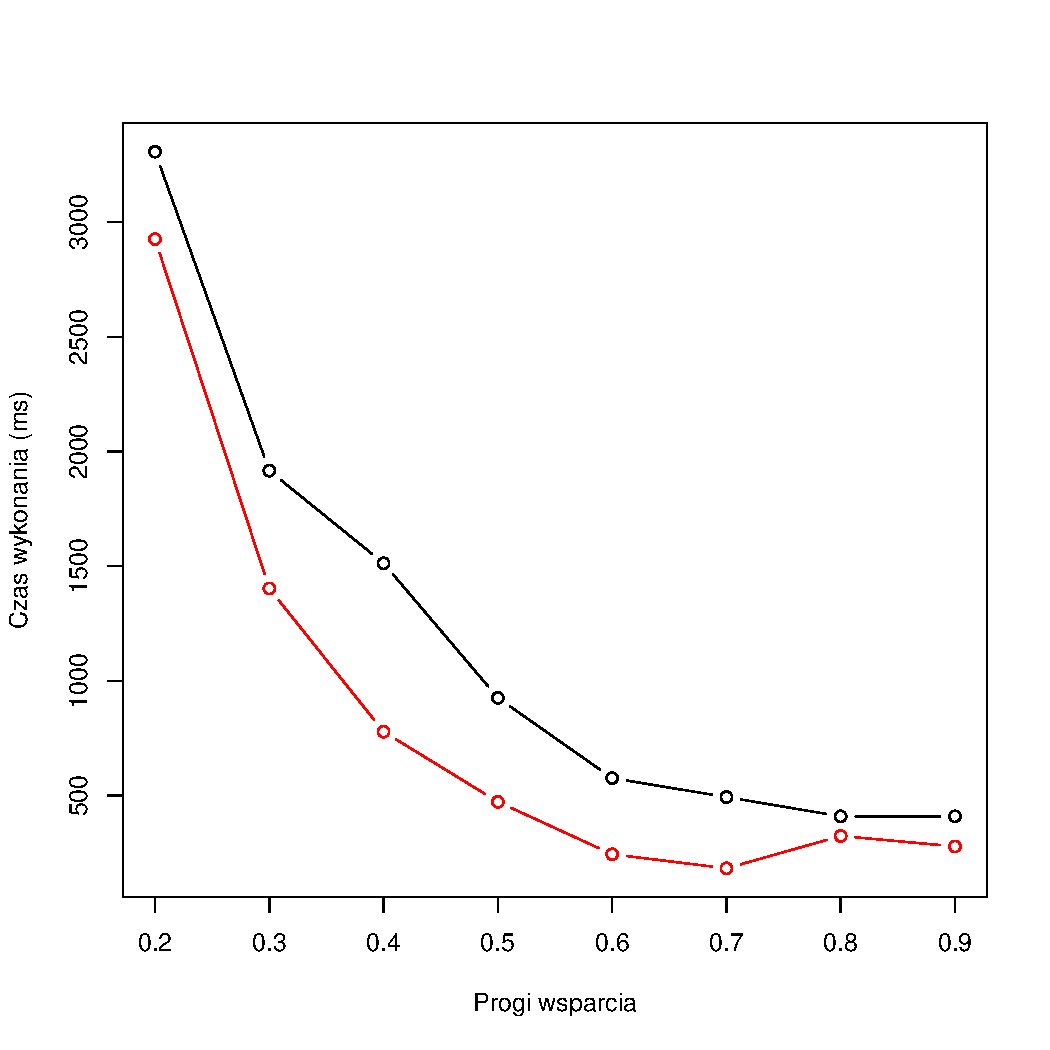
\includegraphics[scale=0.7]{plots/Mushroom.pdf}
\label{plot:mushroom}
\end{figure}

\begin{figure}
\caption{Test dla zbioru House}
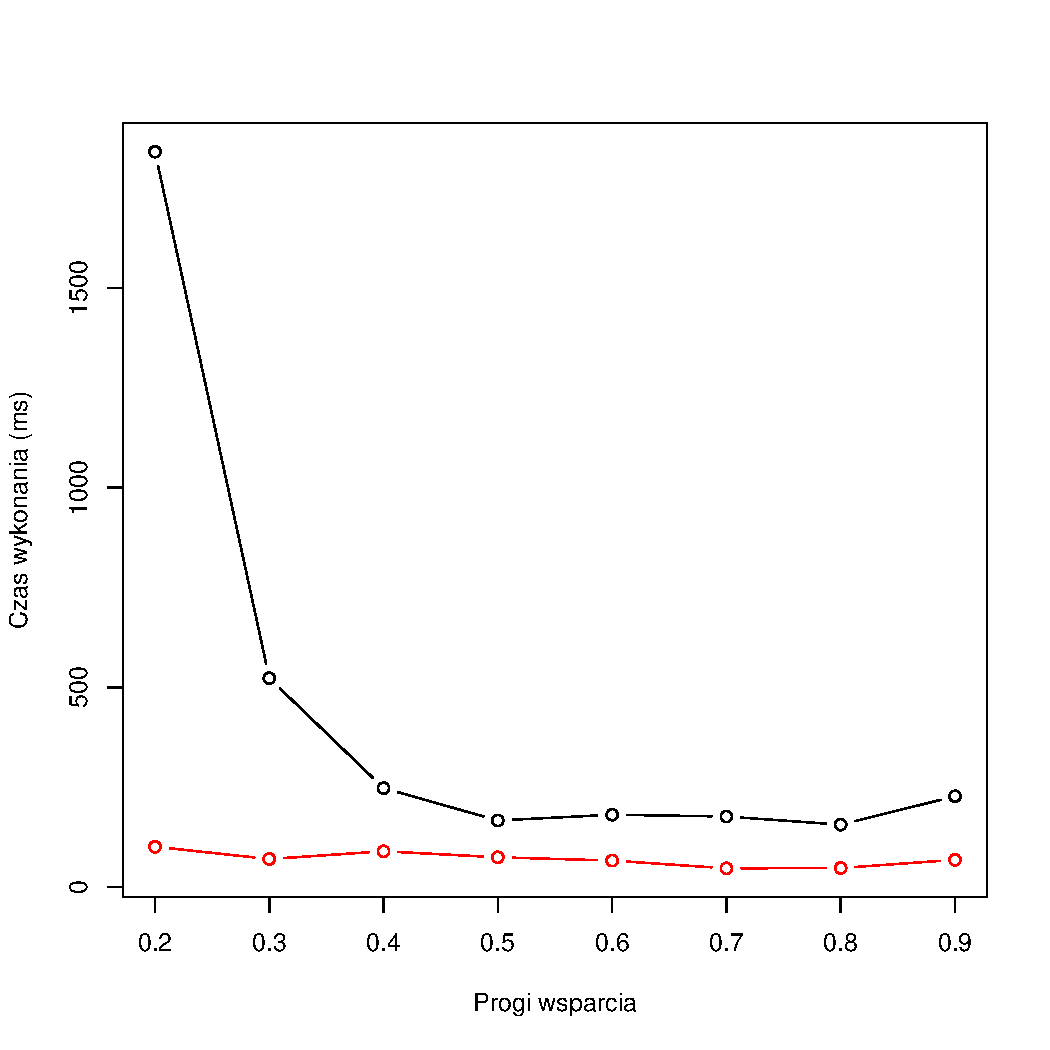
\includegraphics[scale=0.7]{plots/House.pdf}
\label{plot:house}
\end{figure}

\begin{figure}
\caption{Test dla zbioru Promotor}
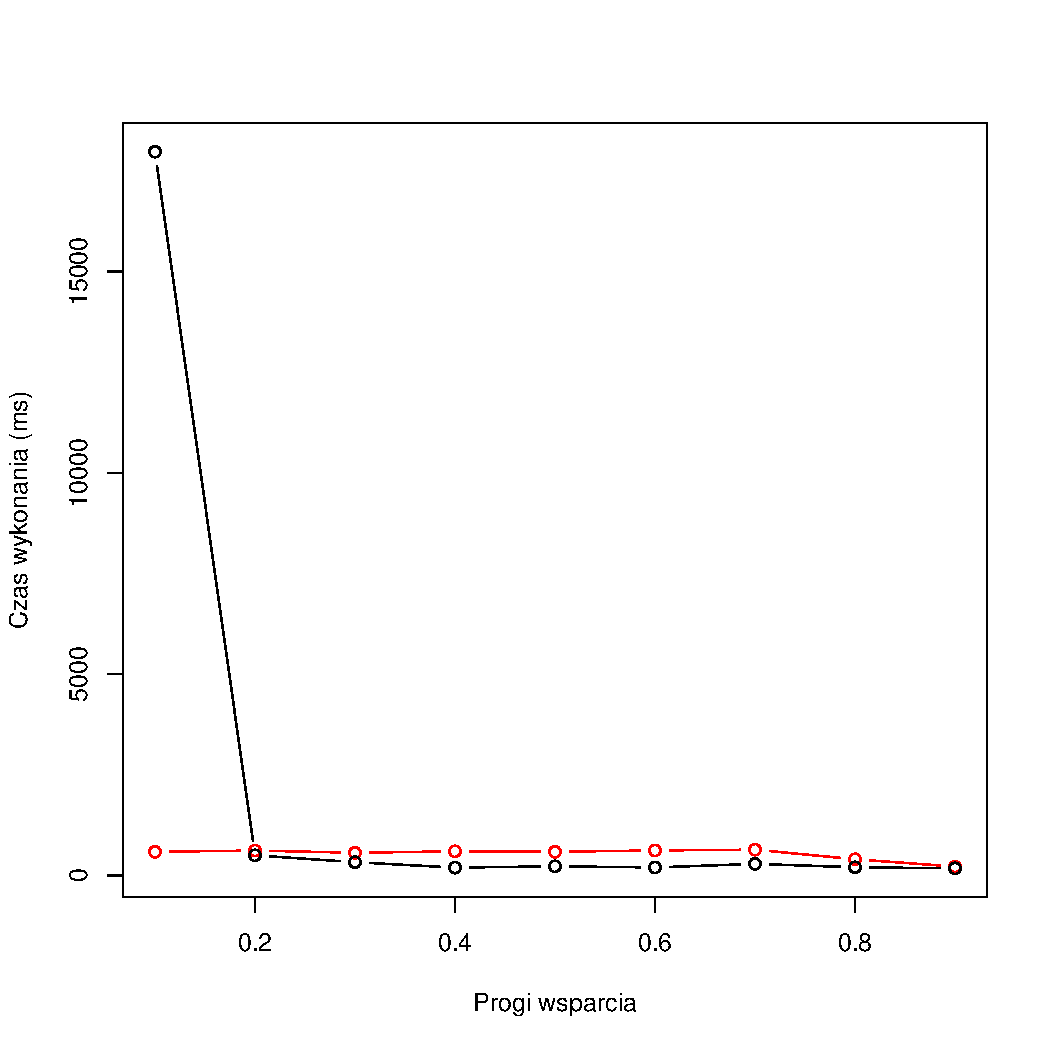
\includegraphics[scale=0.7]{plots/Promotor.pdf}
\label{plot:promotor}
\end{figure}

\begin{figure}
\caption{Test dla zbioru Splice-jxn}
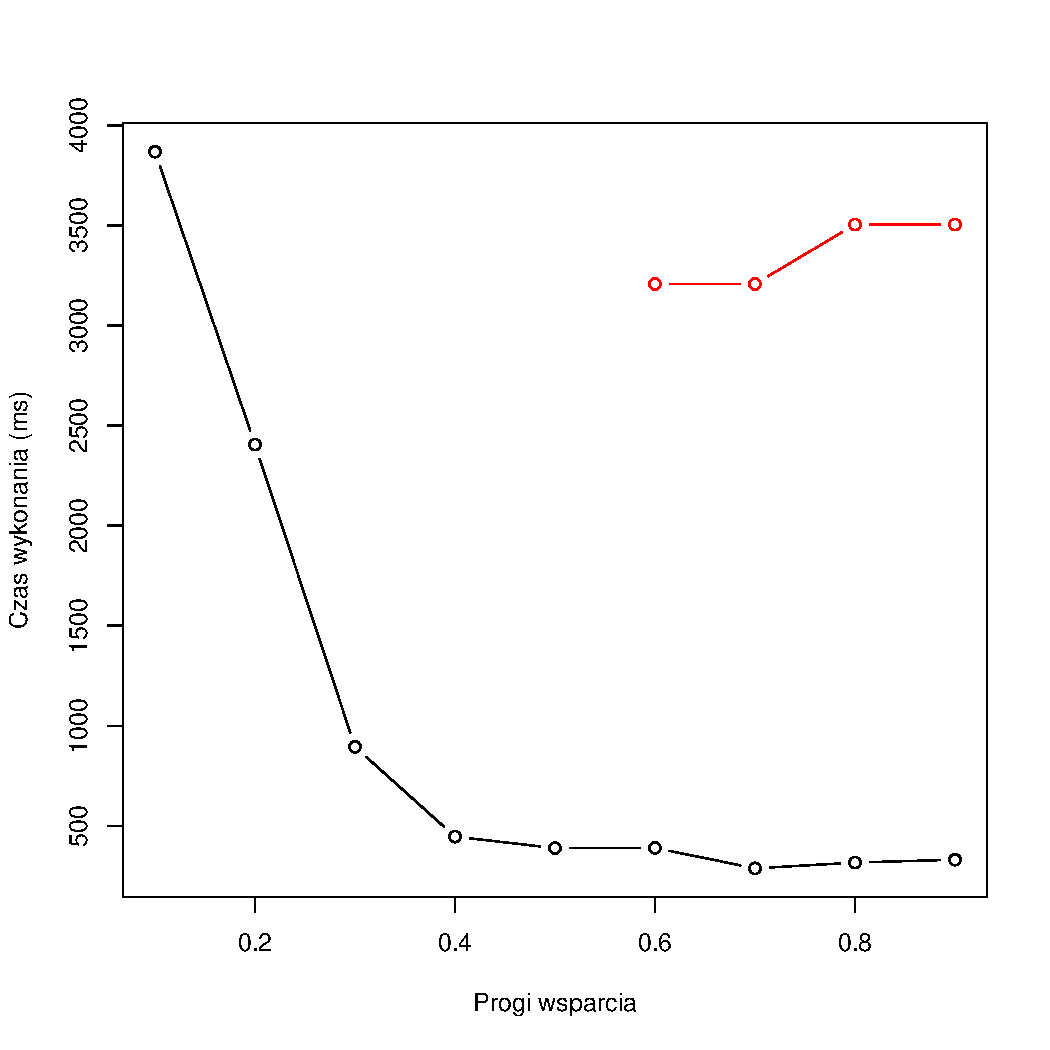
\includegraphics[scale=0.7]{plots/Slice.pdf}
\label{plot:slice}
\end{figure}


\subsection{Profilowanie}

\subsubsection{CHARM}

Wyniki profilowania algorytmu CHARM znajdują się na Rys. \ref{charm:profil}. Tak jak można było się spodziewać, większość czasu program spędził w głównej metodzie algorytmu. Można zauważyć, że aż 10\% czasu procesora zostało zużyte na wyliczanie funkcji skrótu obiektów. Wynika to z tego, że w algorytmie występuje bardzo dużo porównywania zbiorów transakcji, w których występują poszukiwane zbiory częste. Jako, że najszybsze wyszukiwanie w tego typu warunkach gwarantowały kolekcje \emph{HashSet}, to one zostały wykorzystane w tych kluczowych miejscach. Na dole wykresu widać także, że wykorzystanie 13\% czasu procesora związane było z obsługą wielowątkowości. Pomimo nie napisania żadnego specjalnego kodu do obsługi wielu wątków dzięki wykorzystaniu mechanizmu \emph{parallelStream}, który pojawił się w Java 8, w bardzo prosty sposób można zrównoleglić niektóre operacje na kolekcjach, co zostało wykorzystane w projekcie.

\begin{figure}
\caption{Wyniki profilowania algorytmu CHARM}
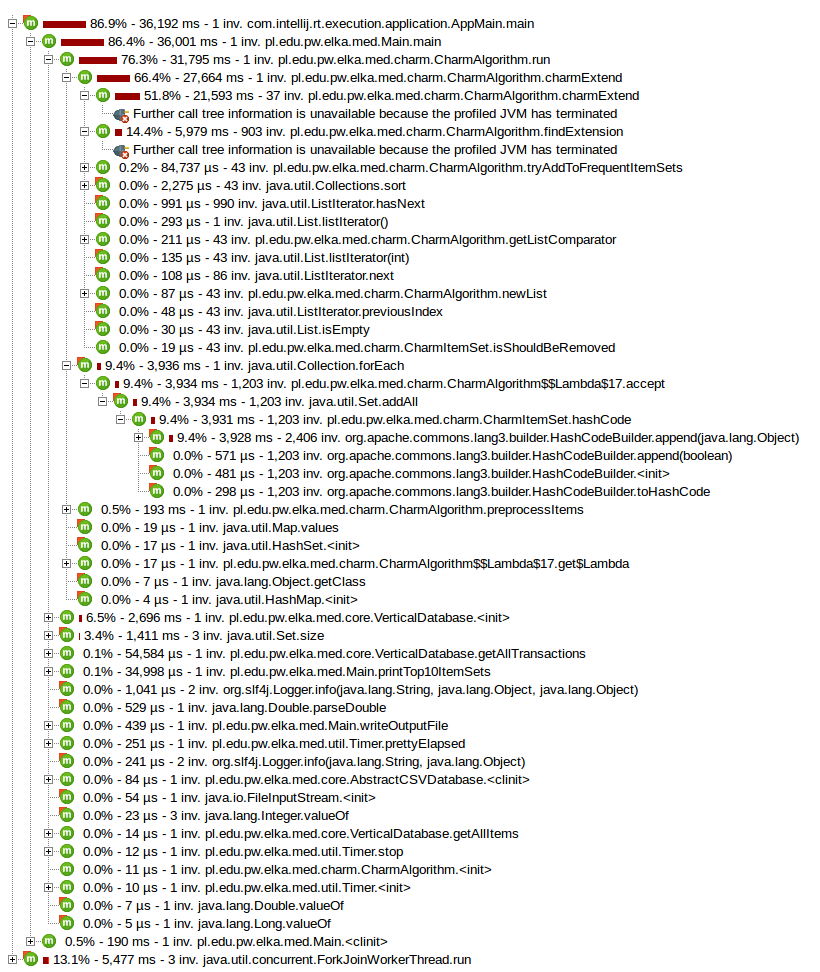
\includegraphics[width=17cm]{res/charm-profi.png}
\label{charm:profil}
\end{figure}

\subsubsection{CLOSET}

Wyniki profilowania algorytmu CLOSET znajdują się na Rys. \ref{closet:profil}.
W sumie większość czasu program spędził w głównej metodzie algorytmu, dlatego że jest to element wywoływany rekurencyjnie.
Można jednak zauważyć wysokie obciążenie funkcji \textit{createDB}, która odpowiadała za tworzenie warunkowych baz danych (na każdym poziomie wywołania funkcji \textit{closet}).
W niej można upatrywać możliwości zwiększenia wydajności, np. poprzez implementację drzewa FP-tree, co sugerują autorzy pracy \cite{closetArt}.

\begin{figure}
\caption{Wyniki profilowania algorytmu CLOSET}
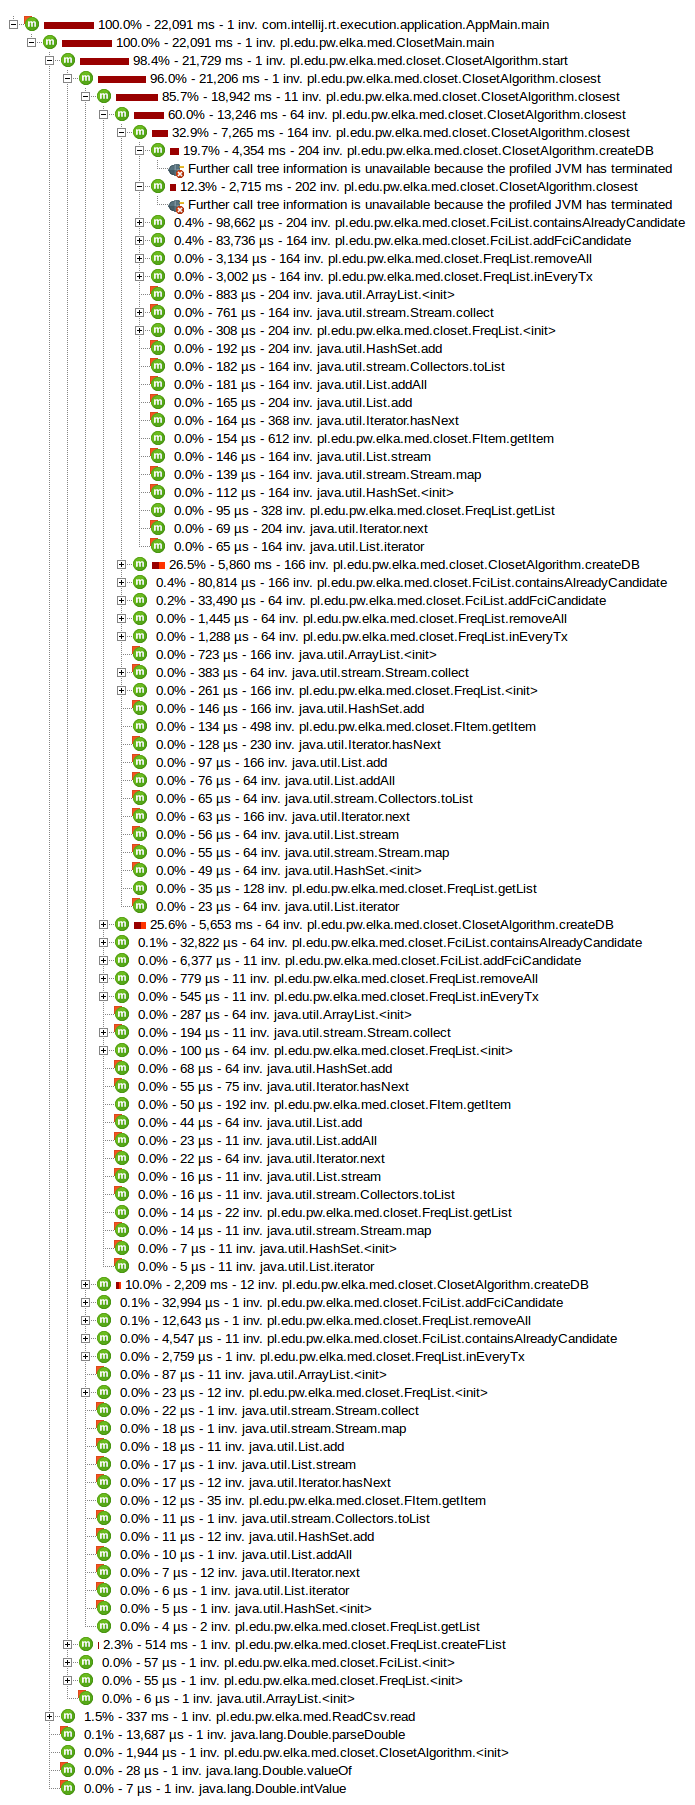
\includegraphics[width=14cm]{res/closet-profi.png}
\label{closet:profil}
\end{figure}